%
% "Building Debian Packages"
% Copyright (C) 2007  Chris Lamb <chris@chris-lamb.co.uk
% Based on a template (C) Daniel Watkins <D.M.Watkins@warwick.ac.uk>
%                         Chris Lamb <chris@chris-lamb.co.uk>
%
%  This program is free software; you can redistribute it and/or modify
%  it under the terms of the GNU General Public License as published by
%  the Free Software Foundation; either version 3 of the License, or
%  (at your option) any later version.
%
%  This program is distributed in the hope that it will be useful,
%  but WITHOUT ANY WARRANTY; without even the implied warranty of
%  MERCHANTABILITY or FITNESS FOR A PARTICULAR PURPOSE.  See the
%  GNU General Public License for more details.
%
%  You should have received a copy of the GNU General Public License
%  along with this program; if not, write to the Free Software
%  Foundation, Inc., 51 Franklin St, Fifth Floor, Boston, MA  02110-1301  USA

\documentclass{beamer}

\usepackage{beamerthemesplit}
\usetheme{Warsaw}

\usepackage{graphicx}
\usepackage{url} 

\usepackage{listings} 
\lstset{basicstyle=\ttfamily}


\title[Building Debian Packages]{Building Debian Packages}
\author[Chris Lamb, WUGLUG]{Chris Lamb\\Warwick University GNU/Linux User Group}
\date{7th November 2007
\newline
\newline

\includegraphics[width=15mm]{debian-logo.png}
\newline
\newline
\tiny{The \LaTeX{} source code for this presentation is licensed under version 3 of the GNU General Public License.}}

\begin{document}

\frame{\titlepage}

%%%%%%%%%%%%%%%%%%%%%%%%%%%%%%%%%%%%%%%%%%%%%%%%%%%%%%%%%%%%%%%%%%%%%%%%%%%%%%%%%%%%%%%%%%
\section{Packaging overview}

    \subsection{When to package}
        \frame {
            \frametitle{When to package}

            \begin{itemize}
                \item Keeping your system 'clean'
                \begin{itemize}
                    \item No `invisible' libraries 
                \end{itemize}
                \item Developing software:
                \begin{itemize}
                    \item \lstinline!/usr/local/! not really good enough
                \end{itemize}
            \end{itemize}
        }

    \subsection{When not to package}
        \frame {
            \frametitle{When not to package}

            \begin{itemize}
                \item Package already exists
                \item Can be generated by helper commands:
                \begin{itemize}
                    \item \lstinline!alien! makes a good job of simple RPMs
                    \item CPAN packages: \lstinline!dh-make-perl --build --notest --cpan \$PACKAGE!
                \end{itemize}
            \end{itemize}
        }

\section{Creating a simple package}

    \subsection{Overview}

    \frame {
        \frametitle{Overview}

        \begin{itemize}
            \item Most packages have two components:
            \begin{enumerate}
                \item An `upstream tarball' (\lstinline!.orig.tar.gz!)
                \begin{itemize}
                    \item Contains the source of the program
                \end{itemize}

                \item A `patch' (\lstinline!diff.gz!)
                \begin{itemize}
                    \item Adds packaging metadata
                \end{itemize}
            \end{enumerate}
            \vskip 1em
            \item Packages can omit the patch - ``Debian native packages''
        \end{itemize}
    }

    \frame {
        \center{ 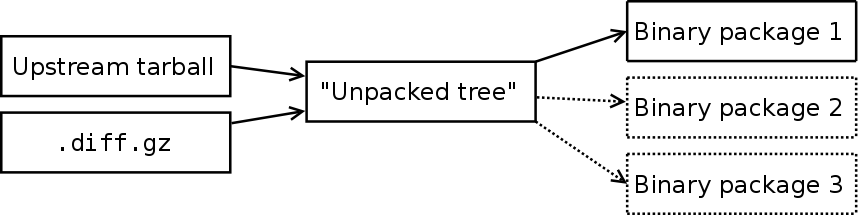
\includegraphics[width=105mm]{overview.png} }
    }

    \subsection{Packaging metadata}

    \frame {
        \frametitle{Packaging metadata}
        \begin{itemize}
            \item All metadata resides in \lstinline!debian/!
            \item Best practice not to modify outside \lstinline!debian/!
            \item Important files:
            \begin{itemize}
                \item \lstinline!debian/control!
                \item \lstinline!debian/changelog!
                \item \lstinline!debian/copyright!
                \item \lstinline!debian/rules!
            \end{itemize}
        \end{itemize}
    }

    \frame {
        \frametitle{\lstinline!debian/control!}
        \begin{itemize}
            \item Contains build and package-dependencies
            \item Consists of:
            \begin{itemize}
                \item One \emph{source} stanza (build dependencies, sections)
                \item One or more \emph{binary} stanzas (install dependencies)
            \end{itemize}
            \center{ 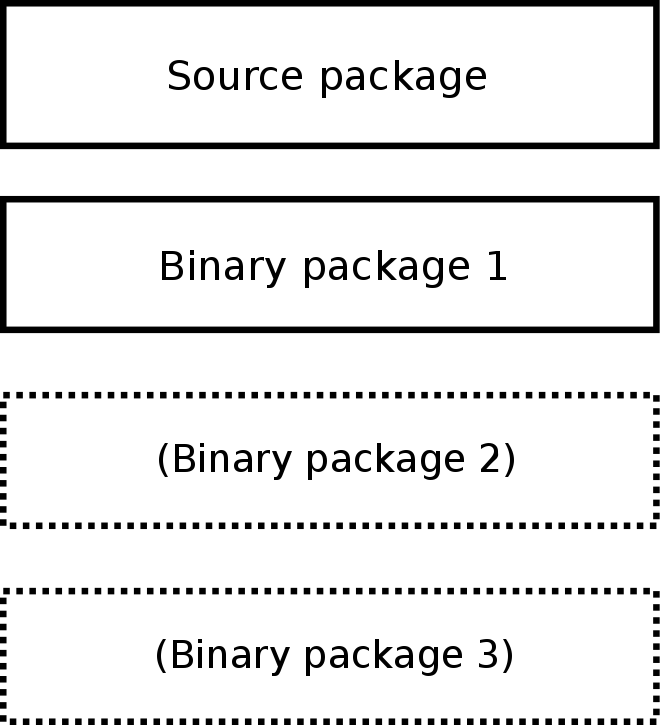
\includegraphics[width=20mm]{control.png} }
            \item Names of source and binary packages in different namespaces
        \end{itemize}
    }

    \frame {
        \begin{itemize}
            \item Typical source stanza:
        \end{itemize}
        \begin{scriptsize}
            \lstinputlisting{control-source.txt}
        \end{scriptsize}
    }

    \frame {
        \begin{itemize}
            \item Typical binary stanzas (some omitted):
        \end{itemize}
        \begin{scriptsize}
            \lstinputlisting{control-binary.txt}
        \end{scriptsize}
    }

    \subsection{\lstinline!debian/changelog!}
    \frame {
        \frametitle{\lstinline!debian/changelog!}
        \begin{itemize}
            \item Contains
                \begin{itemize}
                    \item Source package name
                    \item Source package version
                    \item Source package distribution
                    \item What changed in this version
                \end{itemize}
            \item Picky format - create entries with \lstinline!dch! tool
        \end{itemize}
    }

    \frame {
        \begin{tiny}
            \lstinputlisting{changelog.txt}
        \end{tiny}
    }

    \subsection{\lstinline!debian/rules!}
    \frame {
        \frametitle{\lstinline!debian/rules!}
        \begin{itemize}
        \end{itemize}
    }

    \subsection{Building our first package}
    \frame {
        \frametitle{Building our first package}

        \begin{example}
            \lstinline!dpkg-buildpackage -uc -us!
        \end{example}
    }

\section{Next steps}
    \subsection{Applying patches}
        \frame {
            \frametitle{Applying patches}

            \begin{itemize}
                \item Approaches:
                \begin{itemize}
                    \item Alter upstream tarball
                    \item Make alterations to unpackaged package
                    \item \lstinline!dpatch!
                    \item \lstinline!quilt!
                \end{itemize}
            \end{itemize}
        }

    \subsection{Building in sane environment}
        \frame {
            \frametitle{Building in sane environments}

            \begin{itemize}
                \item Building packages
                \item Advantages:
                \begin{itemize}
                    \item Keep host system clean
                    \item Build for different architectures and distributions
                    \item Prevents accidental linkage
                    \item Reproducible
                \end{itemize}
            \end{itemize}
         }

    \subsection{Lintian and Linda}
        \frame {
            \frametitle{Lintian and Linda}

            \begin{itemize}
                \item Statically checks packages for common errors
                \item Fairly comprehensive: spelling, executable stacks, encodings, etc.
                \item Important that you fix errors
            \end{itemize}

            \begin{block}{Dissecting a Lintian warning}
                \begin{itemize}
                    \item Check Lintian manual
                    \item Google
                    \item \lstinline!dpkg -L lintian | grep "\^/usr/share/lintian/checks/" | xargs grep check-name!
                \end{itemize}
            \end{block}
        }

    \subsection{Sharing your packages}
        \frame {
            \frametitle{Sharing your packages}
            
            \begin{itemize}
                \item Distributing \lstinline!.deb!s vs. repositories
                \item APT repository -- \lstinline!Packages! \lstinline!Sources!
                \item Using \lstinline!dupload! to automate task
            \end{itemize}
        }

        \frame {
            \lstinputlisting{dupload.txt}
        }

    \subsection{Getting them into Debian}
    \frame {
        \frametitle{\lstinline!debian/changelog!}

        \begin{itemize}
            \item sdfds
        \end{itemize}
    }

%%%%%%%%%%%%%%%%%%%%%%%%%%%%%%%%%%%%%%%%%%%%%%%%%%%%%%%%%%%%%%%%%%%%%%%%%%%%%%%%%%%%%%%%%%

\frame {
    \frametitle{Thanks!}
    WUGLUG contact information:
    \begin{itemize}
        \item Website: \url{http://www.wuglug.org.uk}
        \item IRC: {\tt \#wuglug} on {\tt irc.uwcs.co.uk:6667}
        \item Mailing list: \url{https://mailman.warwickcompsoc.co.uk/listinfo/wuglug}
    \end{itemize}
}

\end{document}
